\documentclass[border=5pt]{standalone}
\usepackage{tikz}
\usetikzlibrary{calc, positioning}
\usepackage{amsmath}
\begin{document}
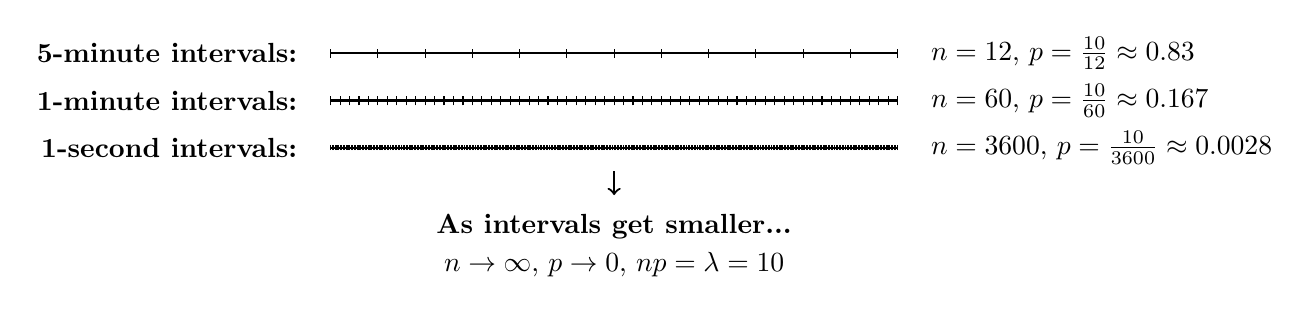
\begin{tikzpicture}[scale=0.6]
% First division: 12 intervals (5 minutes each)
\draw[thick] (0,3) -- (12,3);
\foreach \x in {0,1,...,12}
    \draw (\x,2.9) -- (\x,3.1);
\node[left] at (-0.5,3) {\textbf{5-minute intervals:}};
\node[right] at (12.5,3) {$n = 12$, $p = \frac{10}{12} \approx 0.83$};

% Second division: 60 intervals (1 minute each)
\draw[thick] (0,2) -- (12,2);
\foreach \x in {0,0.2,...,12}
    \draw (\x,1.9) -- (\x,2.1);
\node[left] at (-0.5,2) {\textbf{1-minute intervals:}};
\node[right] at (12.5,2) {$n = 60$, $p = \frac{10}{60} \approx 0.167$};

% Third division: 3600 intervals (1 second each)
\draw[thick] (0,1) -- (12,1);
\foreach \x in {0,0.03333,...,12}
    \draw (\x,0.95) -- (\x,1.05);
\node[left] at (-0.5,1) {\textbf{1-second intervals:}};
\node[right] at (12.5,1) {$n = 3600$, $p = \frac{10}{3600} \approx 0.0028$};

% Arrow showing the limit
\draw[thick,->] (6,0.5) -- (6,0);
\node[below] at (6,-0.2) {\textbf{As intervals get smaller...}};
\node[below] at (6,-1) {$n \to \infty$, $p \to 0$, $np = \lambda = 10$};
\end{tikzpicture}
\end{document}
